
    \documentclass[a4paper,12pt]{article}
    \usepackage{graphicx} 
    \usepackage[utf8]{inputenc}
    \usepackage{longtable}
    \usepackage{booktabs}

    \begin{document}
    \title{Identity Report}
    \maketitle
    \noindent
    \begin{minipage}{0.5\textwidth}
        \large\textbf{Artist:} Michele Sambin\newline
        \large\textbf{Title:}  Il tempo consuma\newline
        \large\textbf{Year:}  1978-01-01\newline
    \end{minipage}
    \hfill
    \begin{minipage}{0.48\textwidth} 
        \centering
        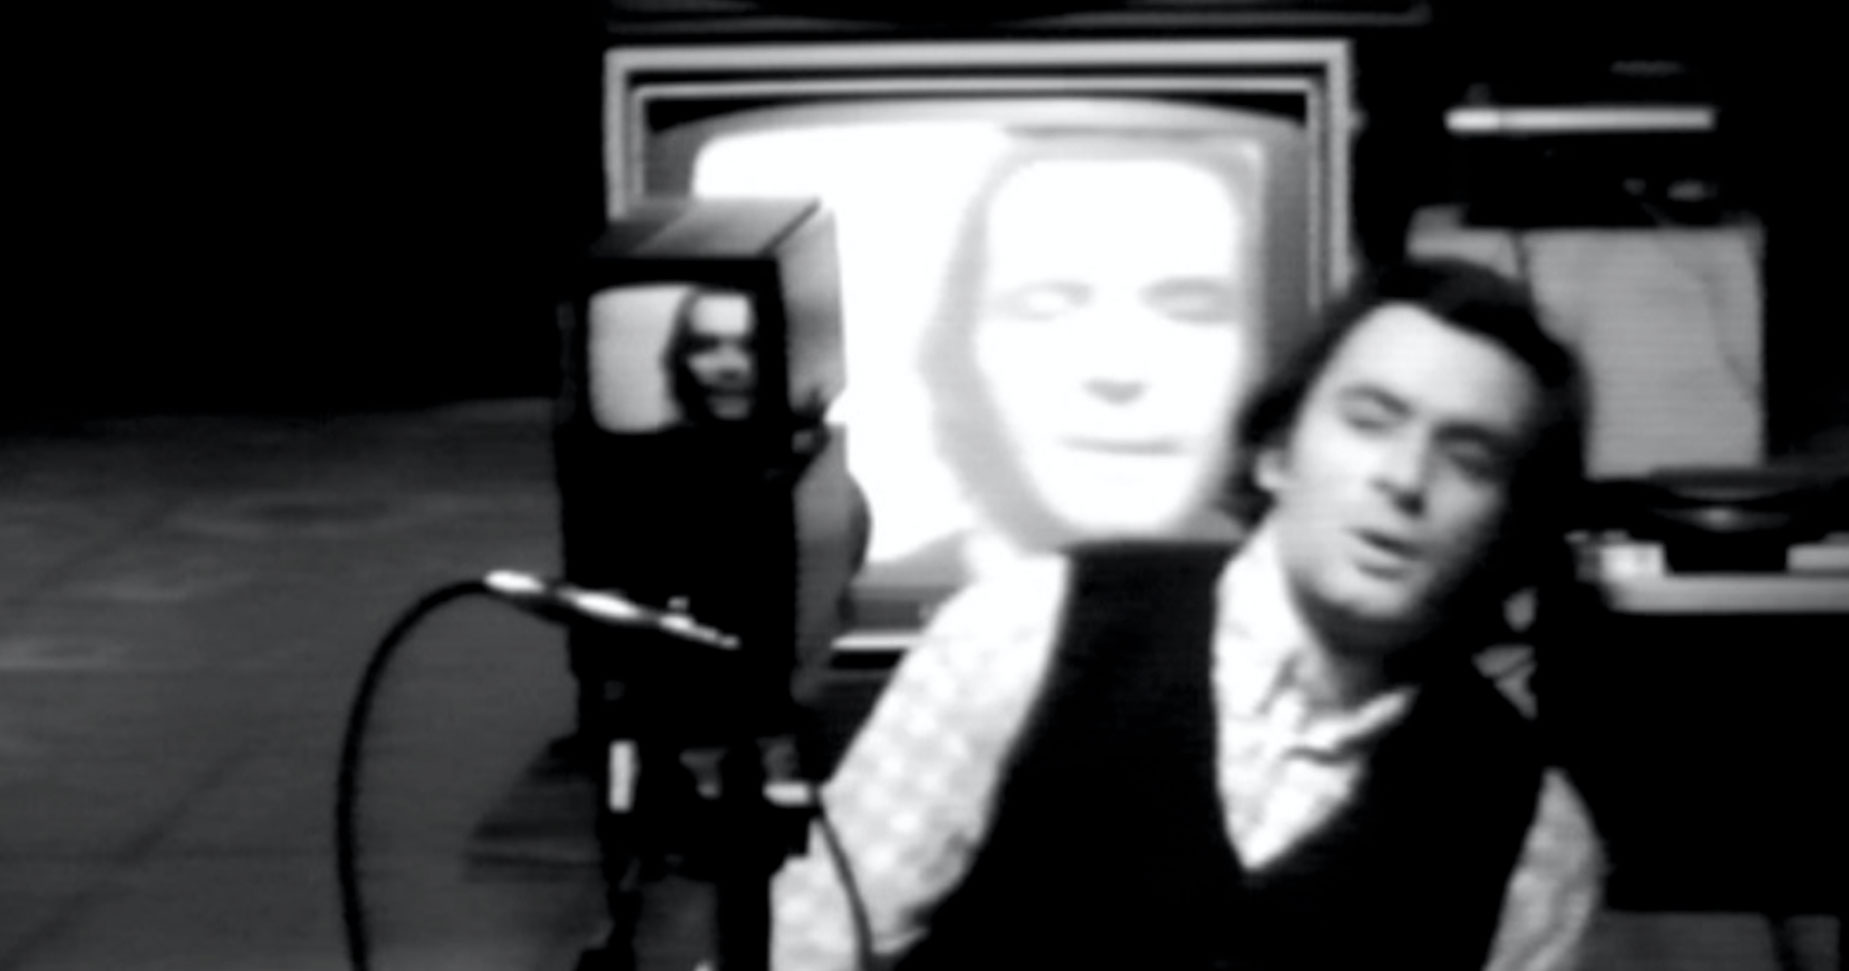
\includegraphics[width=\textwidth]{image.jpg}
    \end{minipage}

    \section*{Description}
    “The passage of time consumes images and sounds.” This phrase, repeated by a "human metronome," evokes a cyclical deterioration of visuals and audio on screen, which gradually lose their initial form and meaning. In 1978, I invented the video loop during an autumn residency at Galleria del Cavallino in Venice, searching for a real-time way to replay video. By linking tape ends into a loop, I achieved a continuous flow with no rewinding. The video loop transformed my artistic approach: it enabled layered, accelerated self-dialogues, creating an evolving, “perpetual motion” where time and self meld in a dynamic continuum. My piece Il tempo consuma is a testament to this effect, with visuals and sounds transforming autonomously. Over time, these shifts blur identity, abstracting human features. Through this process, the loop has redefined both my art and my understanding of time as a layered, vertical moment.

    \section*{Conservation statement}
    

    \section*{Exhibition and Iteration History}
    \begin{longtable}{|p{0.1\textwidth}|p{0.3\textwidth}|p{0.5\textwidth}|} 
    \hline
    \textbf{N} & \textbf{Date} & \textbf{Venue - title} \\ 
    \hline
    \endfirsthead
    n & 1978 & Galleria del Cavallino, Venice, Italy\\\hline n & 1979-01-01 & Fondazione Bevilacqua La Masa, Venice, Italy\\\hline n & 1980-01-01 & Camere Incantate - Royal Palace, Milan, Italy\\\hline n & 2022-02-19 & MICHELE SAMBIN: ARCHÈ/TÉCHNE. IL TEMPO CONSUMA (1978-2022) - Castromediano Museum, Lecce, Italy\\\hline n & 2022-05-16 & Opera Libera - Sala Dei Giganti, Palazzo Liviano, Padua, Italy\\\hline n & 2022-09-30 & Science4All - Complesso Beato Pellegrino, Padua, Italy\\\hline n & 2023-06-15 & Opera Prima Festival - Giardino 2 Torri, Rovigo, Italy\\\hline n & 2024-10-22 & Giardini del Video - Cinema Arsenale, Pisa, Italy\\\hline 

    \end{longtable}
    \end{document}
    